% begin module approximate integration trapezoid
% % % % % % % % % % % % % % % % % % % % % % % % % % % % % % % %
\begin{frame}
\frametitle{Trapezoidal Approximation}
(usually, but not always, better) Obtained by approximating the graph of $f$ by a series of broken lines
through the successive points $(x_i,f(x_i))$. That is, using trapezoids instead of rectangles, giving better accuracy.

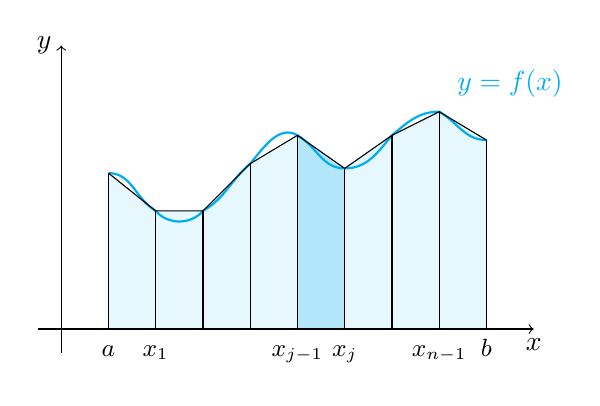
\begin{tikzpicture}[scale=.6]
\coordinate (p1) at (0.7,3);
\coordinate (p2) at (1,3.3);
\coordinate (p3) at (2,2.5);
\coordinate (p4) at (3,2.5);
\coordinate (p5) at (4,3.5);
\coordinate (p6) at (5,4.1);
\coordinate (p7) at (6,3.4);
\coordinate (p8) at (7,4.1);
\coordinate (p9) at (8,4.6);
\coordinate (p10) at (9,4);
\coordinate (p11) at (9.5,4.7);

% The cyan background
\fill[cyan!10] 
  (p2|-0,0) -- (p2) -- (p3) -- (p4) -- (p5) -- (p6) -- (p7) -- (p8) -- (p9) -- (p10) -- (p10|-0,0) -- cycle;
% the dark cyan stripe
\fill[cyan!30] (p6|-0,0) -- (p6) -- (p7) -- (p7|-0,0) -- cycle;
% the curve
\draw[thick,cyan] 
    %(p1) to[out=70,in=180] 
    (p2) to[out=0,in=150] 
    (p3) to[out=-50,in=230] (p4) to[out=30,in=220] 
    (p5) to[out=50,in=150] (p6) to[out=-30,in=180] 
    (p7) to[out=0,in=230] (p8) to[out=40,in=180] 
    (p9) to[out=-30,in=180] (p10); 
    % to[out=0,in=260] (p11);
% the broken line connecting points on the curve
\draw (p2) -- (p3) -- (p4) -- (p5) -- (p6) -- (p7) -- (p8) -- (p9) -- (p10);
% vertical lines and labels
\foreach \n/\texto in {2/{a},3/{x_1},4/{},5/{},6/{x_{j-1}},7/{x_j},8/{},9/{x_{n-1}},10/{b}}
{
  \draw (p\n|-0,0) -- (p\n);
  \node[below,text height=1.5ex,text depth=1ex,font=\small] at (p\n|-0,0) {$\texto$};
}
% The axes
\draw[->] (-0.5,0) -- (10,0) coordinate (x axis);
\draw[->] (0,-0.5) -- (0,6) coordinate (y axis);
% labels for the axes
\node[below] at (x axis) {$x$};
\node[left] at (y axis) {$y$};
% label for the function
\node[above,text=cyan] at (p11) {$y=f(x)$};
\end{tikzpicture}
%\hspace*{2cm}
\uncover<2->{% 
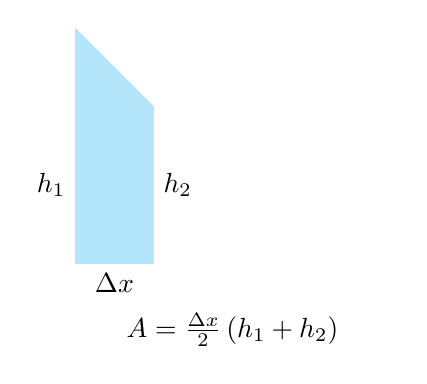
\begin{tikzpicture}[scale=1]
\fill[cyan!30] (3,1) -- (3,4) -- (4,3) -- (4,1) -- cycle;
\node[right,text=black] at (4,2) {$h_2$};
\node[left,text=black] at (3,2) {$h_1$};
\node[below,text=black] at (3.5,1) {$\Delta x$};
\node[below=1cm, align=flush center,text width=4cm] at (5,1.5) {  $\ds A=\frac{\Delta x}{2}\left(h_1+ h_2\right) $};
\end{tikzpicture}
}

\uncover<3->{%
$$\begin{aligned}
\int_a^b f(x)dx &\approx T_n = \sum_{i=1}^n  \frac{\Delta x}{2}(f(x_{i-1})+f(x_i))
\end{aligned}$$
}

\end{frame}
% % % % % % % % % % % % % % % % % % % % % % % % % % % % % % % %
% % % % % % % % % % % % % % % % % % % % % % % % % % % % % % % %
\begin{frame}
\frametitle{Trapezoidal Approximation}
$$\begin{aligned}
\int_a^b f(x)dx &\approx T_n = \sum_{i=1}^n  \frac{\Delta x}{2}(f(x_{i-1})+f(x_i))\\
\uncover<2->{&= \frac{\Delta x}{2}\left[(f(x_0)+f(x_1)) +(f(x_1)+f(x_2))+ \dots +(f(x_{n-1})+f(x_n))\right]\\}
\uncover<3->{&= \frac{\Delta x}2\big[f(x_0)+2f(x_1)+2f(x_2)+\dots +2f(x_{n-1})
+f(x_n)\big].
}
\end{aligned}$$
\uncover<4->{%
\scriptsize 
One may also think of this method as using the average $\frac 1 2(f(x_{i-1})+f(x_i))$ instead of 
$f(x_i^*)$.
}
\end{frame}
% % % % % % % % % % % % % % % % % % % % % % % % % % % % % % % %

% % % % % % % % % % % % % % % % % % % % % % % % % % % % % % % %
\begin{frame}
\frametitle{}
\begin{theorem}[Trapezoid Rule]
 The $ n $'th trapezoidal approximation to $ \ds \int_a^b f(x)\; dx $ is 
 \[
 T_n=\frac{\Delta x}2\left[f(x_0)+2f(x_1)+2f(x_2)+\dots +2f(x_{n-1}+f(x_{n})\right]
 \]
 where $ \Delta x =\frac{b-a}{n}$ and $ x_i=a+i\Delta x. $ \vspace*{4mm}\\
 
 
 Moreover,
 \[
 \lim_{n\to \infty} T_n=\int_a^b f(x)\; dx
 \]
\end{theorem}

% \includegraphics[width=0.9\linewidth]{../../modules/approximate-integration/pictures/T5}
\end{frame}
% % % % % % % % % % % % % % % % % % % % % % % % % % % % % % % %
% end module approximate integration trapezoid
